
\documentclass[9pt,english,ngerman]{scrartcl}
\input{../protokoll_template/template.latex/input/shared_preamble.tex}

\ihead{WS22\\
	30.12.2022} \chead{\textsc{Philipp} Maximilian - 11839611} \ohead{Text zu RDM}

\begin{document}

``Research Data Management'' steht auf drei Säulen Datenhygiene, Datenaufbereitung und
nachhaltige Datensammlung bei Forschungdaten. Oftmals wird über
diese drei Säulen des RDM als Mittel zur Gewährleistung der Qualität und
Integrität von Forschungsdaten. Datenhygiene bezieht sich auf Praktiken
und Prozesse zur Sicherstellung der Genauigkeit, Vollständigkeit und
Konsistenz von Daten, wie z. B. die Validierung der Dateneingabe, die
Überprüfung auf Duplikate und die Verifizierung der Gültigkeit von Datenquellen.
Die Datenaufbereitung umfasst die Umwandlung von Rohdaten in ein brauchbares
Format, z.B. die Bereinigung und Umwandlung von Daten oder die Kombination
mehrerer Datenquellen. Die nachhaltige Datenerfassung im Rahmen von
RDM umfasst die Planung und Umsetzung von Methoden zur langfristigen
Bewahrung und Zugänglichkeit von Forschungsdaten, z.B.
Sicherungs- und Wiederherstellungsverfahren, sowie die Entwicklung
von Datenverwaltungsplänen, die den Lebenszyklus der Daten und
die erforderlichen Schritte zur Aufrechterhaltung ihrer Qualität
und Zugänglichkeit umreißen. Insgesamt besteht das Ziel von RDM darin,
sicherzustellen, dass Forschungsdaten auf eine Art und Weise gesammelt,
verwaltet und aufbewahrt werden, die ihre weitere Nutzung und
Wiederverwendung unterstützt und ihren Wert für die zukünftige Forschung maximiert.

Die ``Framework Policy für Forschungsdatenmanagement an der TU Graz'' soll die
Rahmenbedingungen für ein zukunftfähiges Forschungsdatenmanagement betreiben
kann. Diese Rahmenbedingungen sollen durch geeignete Events, Kurse, Workshops
kultiviert und gepflegt werden. Wo verschiedene Prinzipien, wie ``FAIR'', den
Forschenden übermittelt werden sollen. Der Implementierungsprozess wird mehrere
Jahre dauern und von den verfügbaren Ressourcen abhängen. Das Ziel RDM mit
diesen Richtlinie in der TU zu etablieren basiert auf der Überzeugung, dass
gutes Forschungsdatenmanagement eine wichtige Rolle bei der Förderung
hochwertiger Forschung und der Verwertbarkeit von Forschungsergebnissen spielt.
Aspekten wie der Einhaltung von Best Practices für Reproduzierbarkeit und
Wiederverwendbarkeit, dem verantwortungsvollen Umgang mit Forschungsergebnissen
durch ordnungsgemäße Dokumentation, Speicherung und Verfügbarkeit, der Erhöhung
der Sichtbarkeit der Forschung an der TU Graz sind dabei von höchster
Wichtigkeit. Diese Richtlinien um RDM zu Fördern gelten für alle an der TU Graz
tätigen ForscherInnen, wobei die bestehenden Regelungen zu Open Access,
geistigem Eigentum und Forschungsintegrität beibehalten werden.

\begin{figure}[H]
	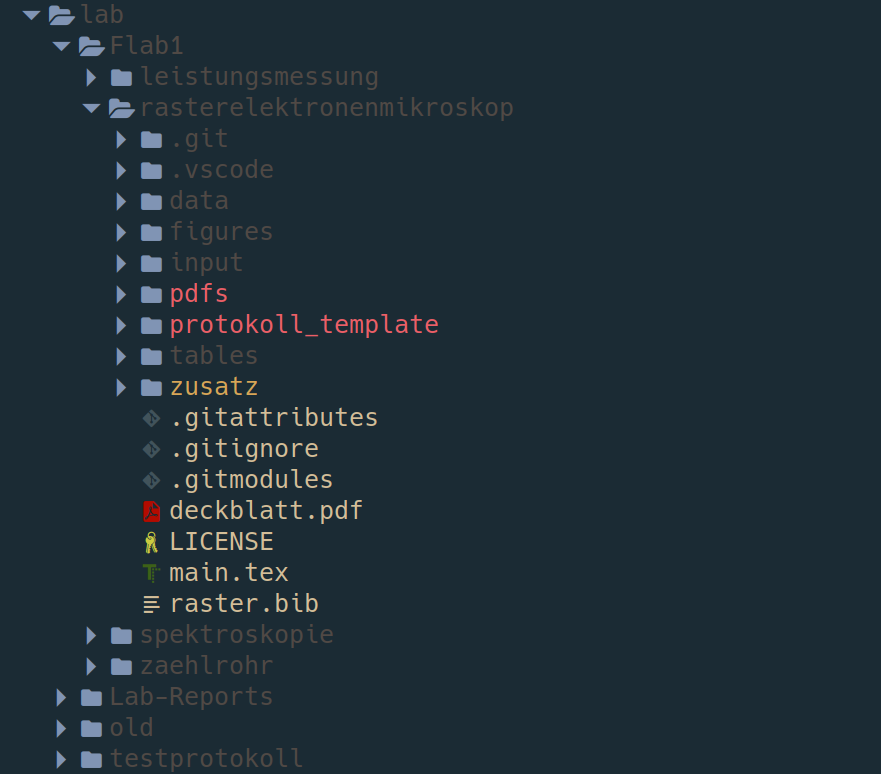
\includegraphics[width=0.45\textwidth]{./foldersmall.png}
	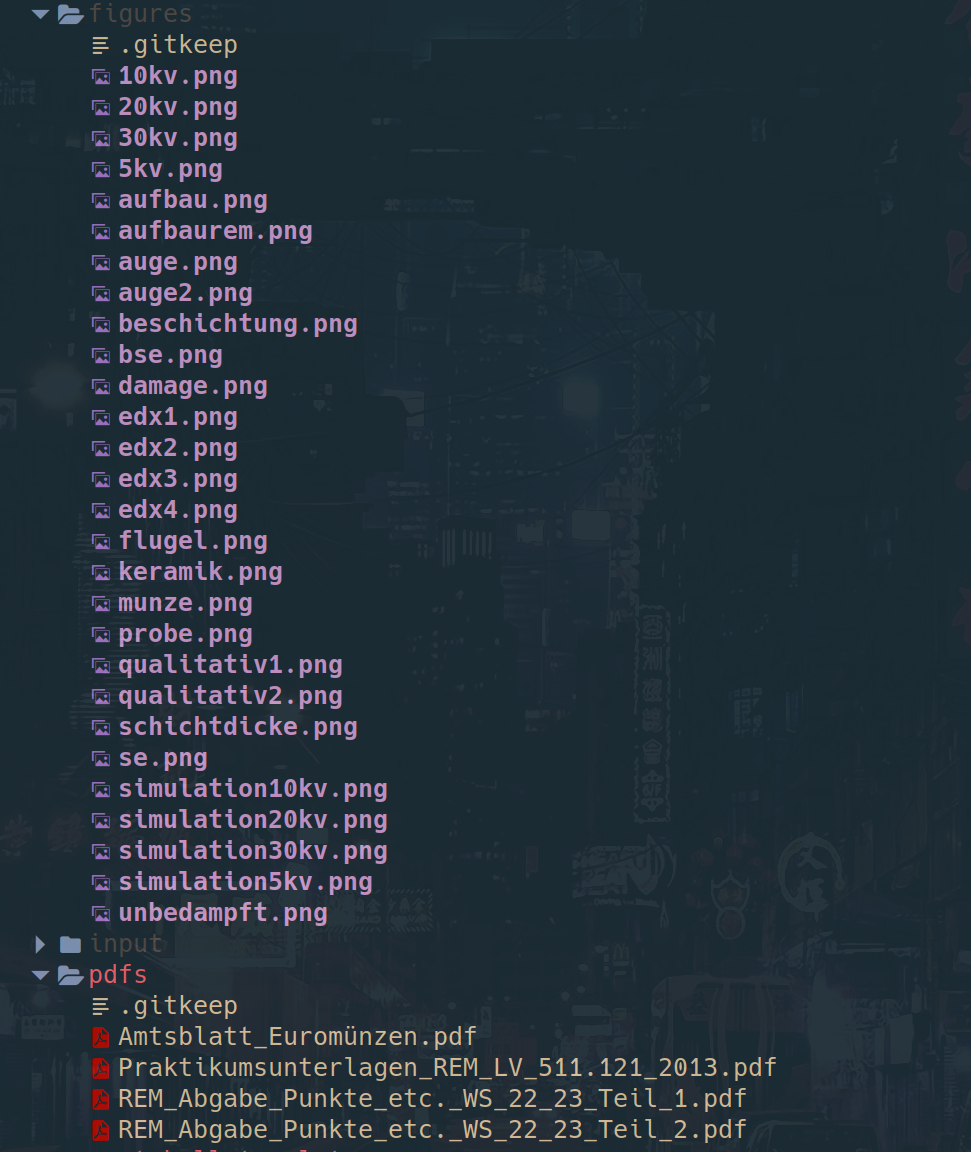
\includegraphics[width=0.45\textwidth,height=6cm]{./picandreferencematerial.png}
\end{figure}

Hier wurde eine übersichtliche Sortierung der Daten gewählt, damit effizientes
Arbeiten durch kategorialer Clustering der Dateien in Bilder, Rohdaten,
Tabellen, PDFs (von Research Material, Angaben, Quellen, usw.) ermöglicht wird.
Wobei eine gute Namensgebung nicht zu vergessen ist, damit ein Zusammenfügen
beim schreiben und einsortieren leichter gemacht wird. Zusätzlich wurde dieses
Protokoll wie alle unserer immer mit einer Version-Control-Software ``GIT''
geschrieben, sodass die ganze Geschichte (Änderungen von wem und was) des
Projekt laufend mit dokumentiert wurde.

\end{document}
